\documentclass[sigplan,nonacm]{acmart}
\usepackage{booktabs}
\setlength{\emergencystretch}{2em}
\settopmatter{printacmref=false,printccs=false,printfolios=true}
\setcopyright{none}
\renewcommand\footnotetextcopyrightpermission[1]{}
\title{Mini-Paper 3: Abelian Sandpile Model}
\author{Carleano Chang}
\email{poching2@illinois.edu}
\affiliation{\institution{University of Illinois Urbana-Champaign}\city{Urbana}\state{Illinois}\country{USA}}
\begin{document}
\begin{abstract}
I optimize the end-to-end computation of an identity sandpile on a $1001\times1001$ Pacman-shaped grid. Precomputed bounds and batch toppling reduce repeated work. Two parallel update designs then expose different tradeoffs in synchronization, symmetry, and vectorization. The selected design combines padded storage, fused red-black updates, reflection symmetry, OpenMP, and SIMD/native compilation. Its mean time is 25.162 seconds, compared with the original single ordinary run of 616.234 seconds, a $24.49\times$ speedup. All recorded performance outputs match the reference PNG, and two final full-grid comparisons also preserve every integer cell value.
\end{abstract}
\maketitle
\noindent\textbf{Code Repository:} \url{https://github.com/Car1eano/fall26-cs598ape-mp3}

\section{Approach and Baseline}
The supplied C program computes the identity of an Abelian sandpile~\cite{starter}. An active cell with at least four grains can topple: it loses four grains and each direct neighbor receives one. Stabilization repeats until no active cell can topple. The identity calculation initializes the grid to six, stabilizes, replaces every value $v$ by $6-v$, and stabilizes again before writing a PNG.

The benchmark uses the supplied Pacman mask and $N=1001$. Only active cells topple, but inactive cells inside the allocated grid receive grains and retain their values through the second initialization and rendering. Grains leaving the grid disappear. I preserve these sink values, not just the visible pattern.

The original commit is \texttt{952c4d3}; the implementation and recorded evidence are preserved in artifact commit \texttt{39bce8b}. Measurements use the course VM: four Intel Xeon Silver 4216 vCPUs at 2.10\,GHz, about 15\,GiB RAM, Ubuntu 26.04.1, and GCC 15.2.0. The baseline already uses \texttt{-O3 -lm -g -Werror}. Parallel builds add \texttt{-fopenmp}; SIMD/native candidates also add \texttt{-march=native}. Thus, enabling \texttt{-O3} is not a new optimization here.

There are 36 ordinary runs across 21 version/thread settings. Reported times are arithmetic means of complete process wall times, including PNG output but excluding compilation. Most settings have two samples; A's simplified core has three. The original and several serial or thread-scaling settings have one. No separate warmup is excluded. Profiling, memory checks, grid dumps, and packaging checks are separate.

A baseline \texttt{perf} profile attributes 99.97\% of sampled user-space CPU cycles to \texttt{stabilize}. Separate phase timers measure 445.051 seconds for the first stabilization, 172.659 for the second, and 0.075 for rendering. This motivates targeting stabilization. Sample percentages are CPU-cycle weights, not wall-time fractions.

\section{Optimizations}
\subsection{Bounds and Batch Toppling}
The original sweeps repeatedly evaluate the circular mask and topple each eligible cell only once per visit. I precompute each row's active interval, removing repeated geometry checks and inactive visits from stabilization. This work-reduction change lowers mean time to 301.623 seconds.

Next, an active cell of value $v\geq4$ topples $q=\lfloor v/4\rfloor$ times at once: subtract $4q$ locally and add $q$ to each existing neighbor. These are legal consecutive topplings; the Abelian property permits the changed order. Mean time becomes 266.574 seconds. Bounds are computed from the input size and mask rather than hardcoded for 1001.

\subsection{Layout and Parallel Update Designs}
Contiguous storage with an outer halo removes directional boundary checks, but alone takes 272.166 seconds, 2.10\% slower than batch toppling. A global two-phase version first records toppling counts, then gathers them into receivers. It avoids concurrent neighbor writes, but costs 848.447 seconds in its single trial. Separate passes and changed propagation order add work; the measurements do not isolate their individual costs.

I therefore compare two parallel branches. \textbf{A} starts from batch toppling without padding. Source rows are grouped by index modulo three. Rows in one group write disjoint three-row neighborhoods; each row retains sequential left-to-right updates. Barriers separate groups, and a shared termination reduction coordinates complete sweeps.

\textbf{B} retains padding and uses checkerboard red-black phases. Each color first records its counts, then receivers gather contributions into their own cells. A barrier separates dependent phases. Restricting gathering to possible receivers avoids whole-grid scans. The serial red-black trial takes 349.891 seconds: better than global two-phase, but still worse than batch toppling.

Both branches use persistent OpenMP teams~\cite{openmp}. With four threads, A averages 96.726 seconds and B 100.325. Table~\ref{tab:threads} compares each branch with its own single-thread implementation. Directly adding a parallel loop to the original scatter update would allow concurrent writes to the same neighbor.

\begin{table}[t]
\caption{Mean wall time in seconds before symmetry. One and two threads have one sample each; four threads have two. Scaling uses each branch's own one-thread time.}
\label{tab:threads}
\centering
\setlength{\tabcolsep}{4pt}
\begin{tabular}{lrrrr}
\toprule
Branch & 1 thread & 2 threads & 4 threads & Scaling \\
\midrule
A & 313.239 & 160.692 & 96.726 & 3.24$\times$ \\
B & 351.297 & 175.759 & 100.325 & 3.50$\times$ \\
\bottomrule
\end{tabular}
\end{table}

\subsection{Symmetry and Scheduling}
For odd $N$, the mask and initialization are symmetric across the middle row. Both branches simulate the upper half including the center, then mirror all final values, including sinks. Mirrored off-center contributions into the center are counted twice; center-to-upper contributions remain single. Even sizes use the full grid because the original integer-centered mask does not have the same reflection symmetry.

At four threads, symmetry reduces A to 49.178 seconds and B to 54.568. A later profile spends 73.09\% of sampled cycles in its worker and about 26.84\% in \texttt{libgomp}; disassembly identifies prominent spin-wait instructions. This suggests investigating scheduling and synchronization, but does not distinguish imbalance from barrier frequency.

Changing A's row schedule from \texttt{static} to \texttt{static,1} distributes rows cyclically and lowers time to 46.205 seconds. A local-flags experiment reduces barriers per sweep from five to four, yet takes 47.883 seconds. Fewer barriers alone do not ensure a gain. Caching fixed values and row pointers, using nonoverlapping row pointers, and separating edge cases simplify A's interior loop; its three-run mean is 39.918 seconds. Adding \texttt{-flto} gives 39.238 seconds, a small observed difference with limited samples.

\subsection{Fused Red-Black Updates and SIMD}
The final change returns to B. For each color, a cell first adds its neighbors' previously published counts to its remainder, then immediately computes its own new count and remainder. Only active cells can produce counts; sinks receive but never topple. Same-color cells are not neighbors, so the phase writes distinct cells and reads counts belonging to the opposite color. A barrier publishes each color's counts before the next phase.

Initially counts are zero. When both colors produce zero counts in a complete sweep, no transfer remains pending; zero counts can also be reused for the second stabilization. Fusing reception and count generation removes separate gathering passes and their barriers. Alone, this version averages 53.421 seconds, but its 48.829--58.013 range makes a small improvement over B symmetry inconclusive.

The independent same-color iterations permit an \texttt{omp simd} loop with a termination reduction~\cite{openmp}. Together with \texttt{-march=native}, this reduces mean time to 25.162 seconds, 52.90\% below fused scalar. GCC reports vectorized stabilization loops using 32-byte and 16-byte vectors. The directive and native flags were enabled together, so I cannot assign separate contributions. Native compilation selects the build machine's instruction set~\cite{gcc}; the performance claim is for this VM, and executables should be rebuilt on the target machine. No explicit architecture intrinsics are used; the scalar fused target remains available without native flags.

\begin{figure}[t]
\centering
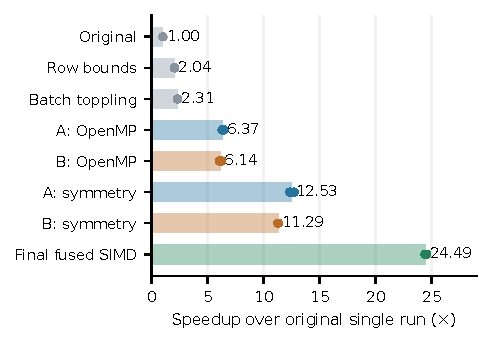
\includegraphics[width=\columnwidth]{figures/stages.pdf}
\caption{Selected cumulative stages at $1001\times1001$. OpenMP stages use four threads. Speedup divides the original single-run time by each stage's mean; all other plotted stages have two runs. A and B are alternatives, not stacked together.}
\label{fig:stages}
\end{figure}

\section{Evaluation and Correctness}
Figure~\ref{fig:stages} summarizes the main gains; Figure~\ref{fig:branches} also retains unsuccessful late experiments. SIMD/native on B's earlier two-phase design takes 55.169 seconds, slightly worse than 54.568, despite compiler-confirmed vectorization. The same combination becomes useful after fusion changes the kernel. Padding and global two-phase also failed in isolation, yet helped organize a later independent update design.

The final runs take 25.088 and 25.236 seconds: mean 25.162, sample standard deviation 0.105. Compared with the original 616.234-second sample, this is $24.49\times$ speedup and 95.92\% less time. The original has no repeated ordinary samples, so its variability is unknown. Small sample counts, development-order batches, and shared-VM load limit statistical conclusions; min--max ranges are observations, not confidence intervals.

All 36 included PNGs match the supplied reference byte for byte. Since distinct sink values can render the same color, numerical checks compare the complete integer grid. The final native design passes two four-thread checks at each of 22 selected sizes between 1 and 201, including odd/even and boundary cases. Two additional $1001\times1001$ comparisons match the original in all 1,002,001 cells.

Small memory checks cover sizes 1, 2, 31, and 32 with one and four threads under Valgrind 3.26.0~\cite{valgrind}. The native executable contains an instruction Valgrind cannot decode, so Memcheck uses the same source with AVX-512 disabled. Native ASan/UBSan checks cover those sizes plus 101 and 102. These checks report no invalid accesses, definite/indirect leaks, or sanitizer errors. At four threads, Memcheck records 864 bytes possibly lost in thread-local-storage allocation stacks and 2,672 still reachable; these are documented rather than called zero leaks. The checks do not prove race freedom.

\begin{figure}[t]
\centering
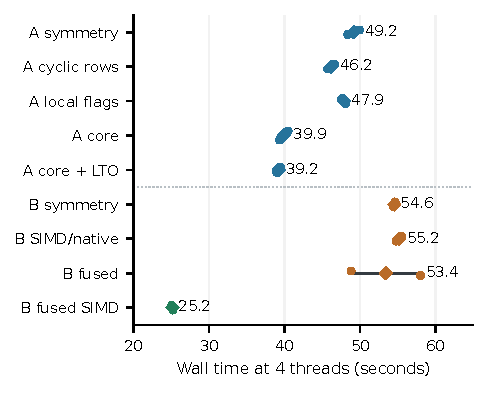
\includegraphics[width=\columnwidth]{figures/branches.pdf}
\caption{Later four-thread variants. Dots are individual runs, diamonds are means, and lines are observed min--max. A core has three runs; other entries have two. B fused has substantial spread; the final fused SIMD/native pair is near 25 seconds.}
\label{fig:branches}
\end{figure}

The artifact preserves the original, intermediate sources, build targets, per-run metadata, CSV summaries, and plotting scripts. OpenMP runs fix dynamic teams off, \texttt{OMP\_PROC\_BIND=close}, and \texttt{OMP\_PLACES=cores}. A source copy without existing binaries, results, or Git metadata builds and runs the default final version in 25.805 seconds with the same PNG. Three randomly selected older variants also pass small execution checks. These are packaging checks, excluded from averages; the installed VM packages were shared, so this is not a fresh-OS test.

\section{Introspection}
The first useful target was repeated work in stabilization, not PNG writing. Bounds and batch toppling reduced that work before parallelization. Later profiles motivated scheduling experiments; the local-flags regression shows that reducing a synchronization count is insufficient without measuring total execution.

The most useful prerequisite was an update design with independent work. Early SIMD and two-phase attempts did not win, while fusion plus SIMD/native did. The evidence supports the combination, not a claim that every component independently accelerates the program. Symmetry also has an explicit scope: odd-sized versions of this mask, with even-size fallback, rather than arbitrary asymmetric domains.

I did not pursue active queues, tiling, narrower cell types, or GPU execution after selecting the final design. They would require additional cost and correctness analysis; this artifact does not establish their benefit. Further work should repeat the baseline, randomize configuration order, and isolate SIMD from native flags before making finer causal claims.

\section{Conclusion}
Work reduction, safe parallel scheduling, reflection symmetry, and fused SIMD/native updates reduce the observed end-to-end runtime from 616.234 to 25.162 seconds. The selected implementation preserves both PNG output and full-grid values in the recorded checks. Failed variants remain reproducible and help explain why changing the update structure mattered more than adding a directive alone.

\begin{thebibliography}{4}
\bibitem{starter}
PRONTOLab. 2026. CS598APE Homework 3 starter code and assignment.
\url{https://github.com/PRONTOLab/598APE-HW3-F26}.
\bibitem{openmp}
OpenMP Architecture Review Board. OpenMP API Specification, Version 5.2.
\url{https://www.openmp.org/spec-html/5.2/openmpse60.html}.
\bibitem{gcc}
Free Software Foundation. GCC 15.2: x86 Options.
\url{https://gcc.gnu.org/onlinedocs/gcc-15.2.0/gcc/x86-Options.html}.
\bibitem{valgrind}
Valgrind Developers. Memcheck: a Memory Error Detector.
\url{https://valgrind.org/docs/manual/mc-manual.html}.
\end{thebibliography}
\end{document}
